\documentclass[tikz,border=10pt]{standalone}
\usepackage{amsmath}
\begin{document}
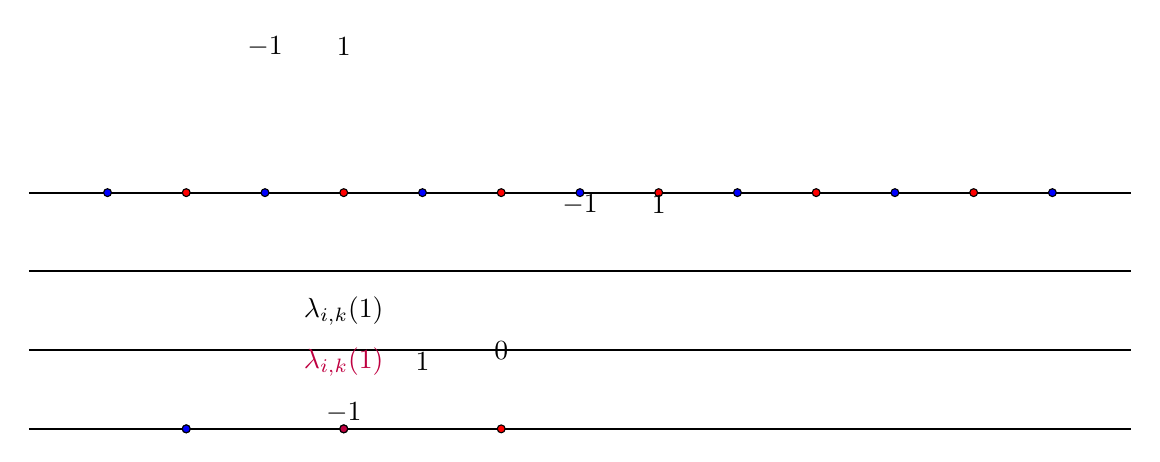
\begin{tikzpicture}[every node/.style={minimum size=1mm-\pgflinewidth, outer sep=0pt}]
    % Draw the horizontal lines
    \foreach \i in {1,...,4} {
        \draw[thick] (-7,1-\i) -- (7,1-\i);
    }
    
    % Blue dots on the left
    \foreach \i in {-6,-4,...,6} {
        \draw[fill=blue] (\i,0) circle (0.5mm);
    }
    
    % Red dots on the right
    \foreach \i in {-5,-3,...,6} {
        \draw[fill=red] (\i,0) circle (0.5mm);
    }
    
    % Label the blue and red dots with -1 and 1
    \foreach \i [evaluate=\i as \y using -\i/2] in {-4,0} {
        \node at (\i, \y - 0.15) {$-1$};
        \node at (\i+1, \y - 0.15) {$1$};
    }
    
    % Add labels in the third and fourth rows
    \node at (-3, -1.5) {$\lambda_{i,k}(1)$};
    \node[color=purple] at (-3, -2.15) {$\lambda_{i,k}(1)$};
    \node at (-2, -2.15) {$1$};
    \node at (-3, -2.8) {$-1$};
    \node at (-1, -2) {$0$};
    
    % Highlight specific conditions in the fourth row
    \foreach \i in {-5,-3,...,0} {
        \draw[fill=red] (\i,-3) circle (0.5mm);
    }
    \draw[fill=purple] (-3,-3) circle (0.5mm);
    \draw[fill=blue] (-5,-3) circle (0.5mm);
    
\end{tikzpicture}
\end{document}